A modelagem fuzzy para controle de ventilação em ambientes fechados foi conduzida com rigor científico, visando garantir clareza, reprodutibilidade e fundamentação teórica. Esta seção detalha todas as etapas do desenvolvimento do sistema fuzzy Mamdani, desde a definição dos universos de discurso até a análise dos resultados, referenciando as imagens e tabelas utilizadas para ilustrar cada conceito.

\subsection{Definição dos Universos de Discurso e Funções de Pertinência}

Os universos de discurso das variáveis foram definidos para cobrir toda a faixa relevante de operação do sistema fuzzy:

\begin{itemize}
    \item Temperatura: $15 \leq x \leq 40$ ($^\circ$C), \texttt{temp\_univ = np.arange(15, 40, 0.1)}
    \item Umidade: $20 \leq x \leq 90$ (\%), \texttt{umid\_univ = np.arange(20, 90, 0.1)}
    \item Pessoas: $0 \leq x \leq 50$, \texttt{pess\_univ = np.arange(0, 50, 0.1)}
    \item Ventilação: $0 \leq x \leq 100$, \texttt{vent\_univ = np.arange(0, 100, 0.1)}
\end{itemize}

Esses intervalos garantem que o sistema fuzzy seja aplicável a diferentes ambientes e condições.

O primeiro passo consistiu na definição dos universos de discurso para as variáveis de entrada (temperatura interna, umidade relativa e número de pessoas) e saída (intensidade da ventilação), conforme apresentado na Tabela~\ref{tab:parametros-triangulares}. Cada variável foi particionada em três conjuntos fuzzy, utilizando funções de pertinência triangulares, de modo a garantir transições suaves e sobreposição adequada entre os estados linguísticos. As funções de pertinência são ilustradas nas Figuras~\ref{fig:fp-temp}, \ref{fig:fp-umid}, \ref{fig:fp-pessoas} e \ref{fig:fp-ventilacao}.

\begin{table}[ht]
\centering
\caption{Parâmetros $(a, b, c)$ das funções de pertinência triangulares}
\label{tab:parametros-triangulares}
\begin{tabular}{llccc}
\hline
\textbf{Variável} & \textbf{Conjunto} & \textbf{a} & \textbf{b} & \textbf{c} \\
\hline
Temperatura (°C) & Baixa   & 15.00 & 21.22 & 27.45 \\
Temperatura (°C) & Média   & 21.22 & 27.45 & 33.67 \\
Temperatura (°C) & Alta    & 27.45 & 33.67 & 39.90 \\
\hline
Umidade (\%)     & Baixa   & 20.00 & 37.48 & 54.95 \\
Umidade (\%)     & Média   & 37.48 & 54.95 & 72.43 \\
Umidade (\%)     & Alta    & 54.95 & 72.43 & 89.90 \\
\hline
Pessoas          & Poucas  & 0.00  & 12.48 & 24.95 \\
Pessoas          & Moderado& 12.48 & 24.95 & 37.43 \\
Pessoas          & Muitas  & 24.95 & 37.43 & 49.90 \\
\hline
Ventilação       & Fraca   & 0.00  & 24.98 & 49.95 \\
Ventilação       & Moderada& 24.98 & 49.95 & 74.93 \\
Ventilação       & Forte   & 49.95 & 74.93 & 99.90 \\
\hline
\end{tabular}
\end{table}


A função de pertinência triangular é definida por:

\begin{equation}
\mu_{A}(x) =
\begin{cases}
0, & x \leq a \\
\frac{x-a}{b-a}, & a < x \leq b \\
\frac{c-x}{c-b}, & b < x < c \\
0, & x \geq c
\end{cases}
\end{equation}

onde $a$, $b$ e $c$ são os parâmetros do conjunto fuzzy.

As curvas de pertinência para cada variável são apresentadas nas Figuras~\ref{fig:fp-temp} (temperatura), \ref{fig:fp-umid} (umidade), \ref{fig:fp-pessoas} (pessoas) e \ref{fig:fp-ventilacao} (ventilação).

% Curvas de pertinência (nomes conferidos conforme imagens geradas pelo notebook mamdani2)
\begin{figure}[ht]
    \centering
    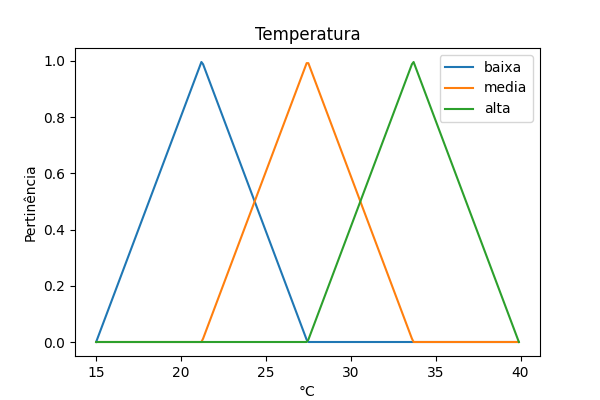
\includegraphics[width=0.48\textwidth]{../img/fp_temp_mamdani2.png}
    \caption{Funções de pertinência triangulares para a variável \textbf{temperatura interna}.}
    \label{fig:fp-temp}
\end{figure}

\begin{figure}[ht]
    \centering
    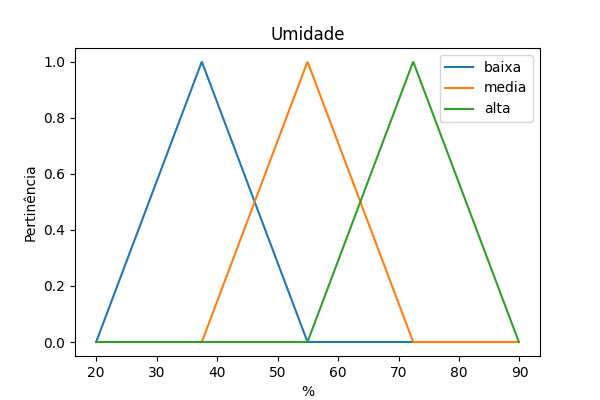
\includegraphics[width=0.48\textwidth]{../img/fp_umid_mamdani2.png}
    \caption{Funções de pertinência triangulares para a variável \textbf{umidade relativa}.}
    \label{fig:fp-umid}
\end{figure}

\begin{figure}[ht]
    \centering
    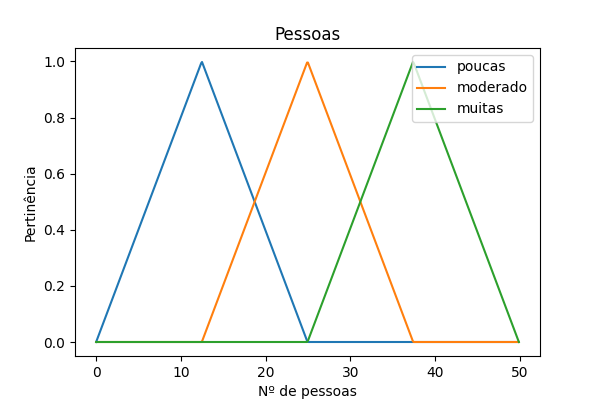
\includegraphics[width=0.48\textwidth]{../img/fp_pessoas_mamdani2.png}
    \caption{Funções de pertinência triangulares para a variável \textbf{número de pessoas}.}
    \label{fig:fp-pessoas}
\end{figure}

\begin{figure}[ht]
    \centering
    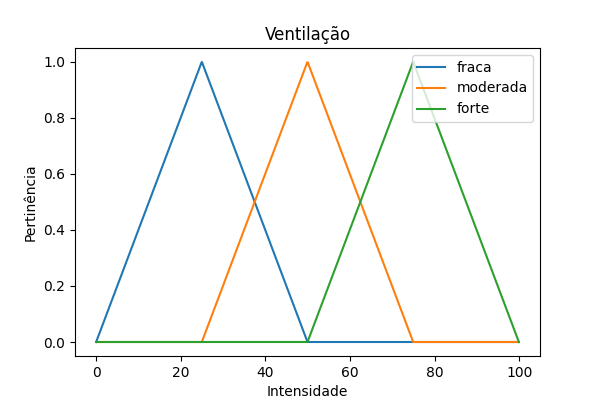
\includegraphics[width=0.48\textwidth]{../img/fp_ventilacao_mamdani2.png}
    \caption{Funções de pertinência triangulares para a variável \textbf{ventilação (saída)}.}
    \label{fig:fp-ventilacao}
\end{figure}


\subsection{Base de Regras Fuzzy}

A base de regras fuzzy foi construída com base em princípios de conforto térmico e conhecimento prático, conforme detalhado na literatura~\cite{ross2010fuzzy}. As regras estabelecem relações qualitativas entre as variáveis de entrada e a intensidade de ventilação recomendada, utilizando operadores fuzzy clássicos (mínimo para AND, máximo para OR):

\begin{itemize}
    \item Se \textbf{temperatura} é \textit{alta} OU \textbf{umidade} é \textit{alta} OU \textbf{pessoas} são \textit{muitas}, então \textbf{ventilação} é \textit{forte}.
    \item Se \textbf{temperatura} é \textit{média} E \textbf{umidade} é \textit{média} E \textbf{pessoas} são \textit{moderadas}, então \textbf{ventilação} é \textit{moderada}.
    \item Se \textbf{temperatura} é \textit{baixa} E \textbf{umidade} é \textit{baixa} E \textbf{pessoas} são \textit{poucas}, então \textbf{ventilação} é \textit{fraca}.
    \item Se \textbf{temperatura} é \textit{alta} E \textbf{umidade} é \textit{baixa}, então \textbf{ventilação} é \textit{moderada}.
    \item Se \textbf{temperatura} é \textit{média} E \textbf{pessoas} são \textit{muitas}, então \textbf{ventilação} é \textit{forte}.
    \item Se \textbf{umidade} é \textit{alta} E \textbf{pessoas} são \textit{poucas}, então \textbf{ventilação} é \textit{moderada}.
    \item Se \textbf{temperatura} é \textit{baixa} OU \textbf{umidade} é \textit{baixa}, então \textbf{ventilação} é \textit{fraca}.
    \item Se \textbf{pessoas} são \textit{moderadas} E \textbf{umidade} é \textit{média}, então \textbf{ventilação} é \textit{moderada}.
    \item Se \textbf{temperatura} é \textit{média} E \textbf{umidade} é \textit{alta}, então \textbf{ventilação} é \textit{forte}.
\end{itemize}


\subsection{Fuzzificação das Entradas}

A fuzzificação constitui a primeira etapa do processamento em sistemas fuzzy, sendo responsável por converter os valores numéricos (crisp) das variáveis de entrada em graus de pertinência nos conjuntos fuzzy previamente definidos. No sistema desenvolvido, cada variável de entrada --- temperatura interna, umidade relativa e número de pessoas --- é associada a três conjuntos fuzzy linguísticos (por exemplo, \textit{baixa}, \textit{média} e \textit{alta} para temperatura e umidade; \textit{poucas}, \textit{moderado} e \textit{muitas} para pessoas).

% Para cada valor de entrada, calcula-se o grau de pertinência em cada conjunto fuzzy por meio das funções de pertinência triangulares, conforme os parâmetros apresentados na Tabela~\ref{tab:parametros-triangulares}. O resultado desse processo é um vetor de graus de pertinência para cada variável, refletindo o quanto cada valor pertence a cada estado linguístico.

% A Tabela~\ref{tab:fuzzificacao} apresenta os graus de pertinência obtidos para cada cenário simulado, evidenciando como a fuzzificação permite representar incertezas e transições suaves entre os estados das variáveis. Esses graus de pertinência são então utilizados na etapa de inferência fuzzy, possibilitando a avaliação das regras e a obtenção de uma resposta interpretável pelo sistema.


\subsection{Inferência Mamdani e Agregação}

A inferência Mamdani utiliza operadores fuzzy para combinar os graus de pertinência das entradas conforme as regras. Os principais operadores utilizados são:

\begin{itemize}
    \item \textbf{AND (mínimo):}
    \begin{equation}
        \mu_{A \cap B}(x) = \min\left(\mu_A(x), \mu_B(x)\right)
    \end{equation}
    \item \textbf{OR (máximo):}
    \begin{equation}
        \mu_{A \cup B}(x) = \max\left(\mu_A(x), \mu_B(x)\right)
    \end{equation}
\end{itemize}

A agregação das saídas das regras é feita por:

\begin{equation}
\mu_{\text{Saída}}(x) = \max_{i} \left( \min\left(\alpha_i, \mu_{B_i}(x)\right) \right)
\end{equation}

onde $\alpha_i$ é o grau de ativação (firing strength) da $i$-ésima regra e $\mu_{B_i}(x)$ é a função de pertinência da saída da regra.

\subsection{Técnicas de Defuzzificação}

As principais técnicas de defuzzificação utilizadas são:

\begin{itemize}
    \item \textbf{Centroide (Center of Area):}
    \begin{equation}
        y^* = \frac{\int_{a}^{b} y \cdot \mu_{\text{Saída}}(y) \, dy}{\int_{a}^{b} \mu_{\text{Saída}}(y) \, dy}
    \end{equation}
    \item \textbf{Média do Máximo (Mean of Maximum):}
    \begin{equation}
        y^* = \frac{1}{n} \sum_{i=1}^{n} y_i, \quad \text{onde } \mu_{\text{Saída}}(y_i) = \max \mu_{\text{Saída}}(y)
    \end{equation}
    \item \textbf{Bissetriz:}
    \begin{equation}
        \int_{a}^{y^*} \mu_{\text{Saída}}(y) \, dy = \frac{1}{2} \int_{a}^{b} \mu_{\text{Saída}}(y) \, dy
    \end{equation}
\end{itemize}
